\section{Experiments Done}

\subsection{Preliminary Test}

This section serves as a baseline. Here, the game is played randomly, without using any training algorithm. Here are the results:

\begin{figure}[H] %h forces the figure to be inserted right here
    \centering
    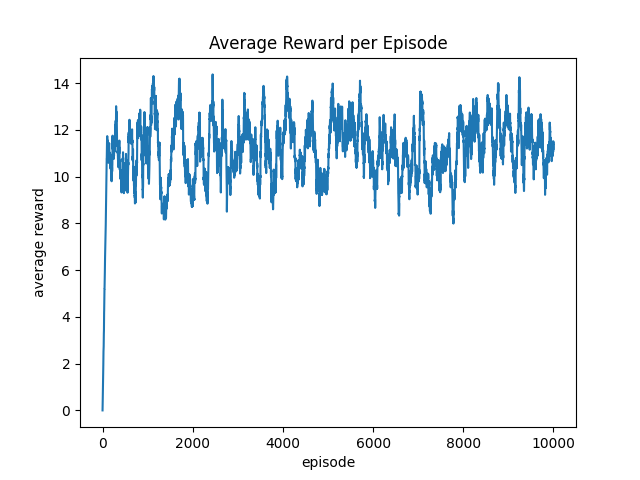
\includegraphics[width=0.75\linewidth]{random-action.png}
    \caption{Baseline Testing Results}
\end{figure}

Looking at the graph, we can see that the average reward are very low.
\subsection{Airi's Experiments - Q-Learning}


% For Q-Learning, she assumed that when the number of episodes gets close to 1000, the pole is balanced upright by the agent choosing to move the cart left or right, while making sure the cart's center not disappear from the screen. 
% The environment is set up as mentioned in the proposal, and in this case, $\gamma = 0.9$, $\alpha = 0.5$, and $\epsilon = 0.5$ for the parameters.  

% For one run of 1000 episodes, here are her current results. Note that due to the random nature of taking actions, each run will produce a different graph.

% \begin{figure}[H] %h forces the figure to be inserted right here
%     \centering
%     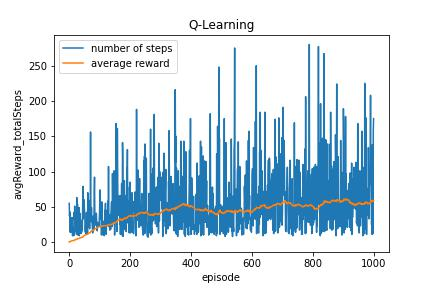
\includegraphics[width=1\linewidth]{q-learning-average-1k.png}
%     \caption{Q-Learning Results Over 1000 Episodes}
% \end{figure}

% Looking at the graph, we can see that the average rewards reached a plateau of approximately 50 after about 200 episodes, this shows that the agent is indeed being trained to
% take more optimal actions as the number of episodes increased.

\subsection{Khoi's Experiments - SARSA Learning}
For SARSA Learning, Khoi is also implementing an $\epsilon$ greedy method. For his setup, the hyperparameters are: $\epsilon = 0.5$; $\gamma = 0.9$; and $\alpha = 0.5$

Addtionally, Khoi is also implementing three differement decaying methods for the $\epsilon$ hyperparameter. These methods will be explained further in the \textbf{General Analysis} section, with \textbf{Hypothesis 2}.

For one run of 10000 episodes, with $\epsilon$ kept static at 0.5, here are his current results. Note that due to the random nature of taking actions, each run will produce a different graph.

\begin{figure}[H] %h forces the figure to be inserted right here
    \centering
    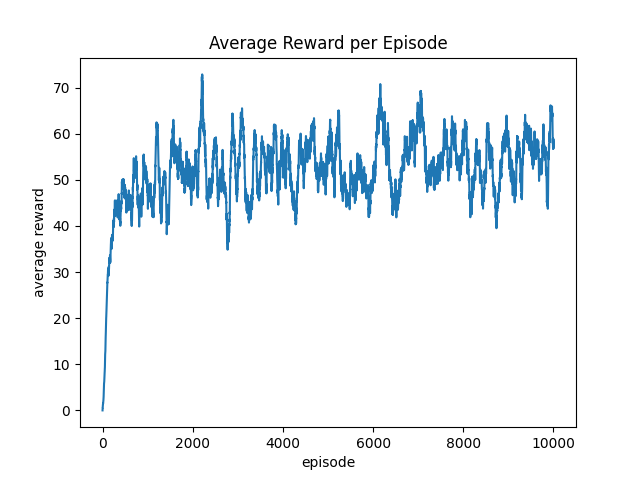
\includegraphics[width=0.75\linewidth]{sarsa-average-10k-epsilon05.png}
    \caption{SARSA Results Over 10000 Episodes, Static $\epsilon$}
\end{figure}

Looking at the graph, we can see that the average rewards reached a plateau of approximately 60 after about 1000 to 1500 episodes, this shows that the agent is indeed being trained to
take more optimal actions as the number of episodes increased. Compared to the baseline results, the average reward are much higher.

% With $\epsilon$ decaying with the function $\epsilon*(\frac{1}{episodes})$, a run will look like so:

% \begin{figure}[H] %h forces the figure to be inserted right here
%     \centering
%     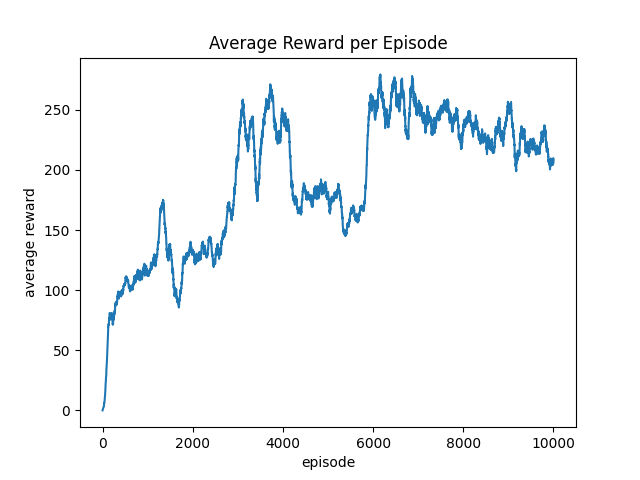
\includegraphics[width=1\linewidth]{sarsa-average-10k-epsilon05decay-run3.png}
%     \caption{SARSA Results Over 10000 Episodes, 1/Episodes Decay}
% \end{figure}

% And finally, with exponential decay of $\epsilon$, a run looks like so:

% \begin{figure}[H] %h forces the figure to be inserted right here
%     \centering
%     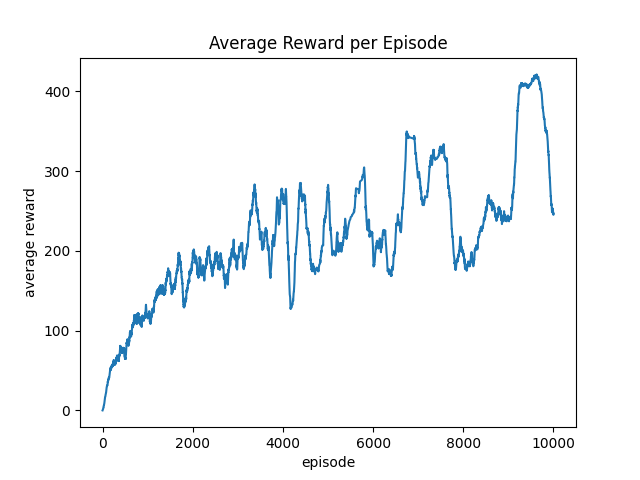
\includegraphics[width=1\linewidth]{sarsa-average-10k-epsilon05exponential-decay-run3.png}
%     \caption{SARSA Results Over 10000 Episodes, Exponential decay}
% \end{figure}